\documentclass[a4paper,11pt]{report}
%%%%%%%%%%%%%%%%%%%%%%%%%%%%
% University of Sussex thesis template
%%%%%%%%%%%%%%%%%%%%%%%%%%%%
% Modification History
%
% Based on usthesis.cls by Jonathon Read
% http://www.cogs.susx.ac.uk/users/jlr24/latex.html
% Modified by Anthony Smith, Feb 2007
% Incorporated into single thesis.tex file, Anthony Smith, 30 June 2008
% Minor alterations to page numbering, AJS, 25 July 2008
% New alternative hyperref options for print version, AJS, 11 Sep 2008
% "DRAFT" on header, AJS, 12 Sep 2008
%%%%%%%%%%%%%%%%%%%%%%%%%%%%
\usepackage{lmodern}
\usepackage{amsmath}


%%%%%%%%%%%%%%%%%%%%%%%%%%%%
% LINE SPACING
\newcommand{\linespacing}{1.5}
\renewcommand{\baselinestretch}{\linespacing}
%%%%%%%%%%%%%%%%%%%%%%%%%%%%


%%%%%%%%%%%%%%%%%%%%%%%%%%%%
% BIBLIOGRAPHY STYLE
\usepackage{natbib}
% \bibliographystyle{plain} for [1], [2] etc.
\bibliographystyle{apalike}
%%%%%%%%%%%%%%%%%%%%%%%%%%%%


%%%%%%%%%%%%%%%%%%%%%%%%%%%%
% OTHER FORMATTING/LAYOUT DECLARATIONS
% Graphics
\usepackage{graphicx,color}
\graphicspath{./figures}
\usepackage{epstopdf}
\usepackage[british]{babel}
% The left-hand-side should be 40mm.  The top and bottom margins should be
% 25mm deep.  The right hand margin should be 20mm.
\usepackage[a4paper,top=2.5cm,bottom=2.5cm,left=4cm,right=2cm,headsep=10pt]{geometry}
\flushbottom
% Pages should be numbered consecutively thorugh the main text.  Page numbers
% should be located centrally at the top of the page.
\usepackage{fancyhdr}
\fancypagestyle{plain}{
	\fancyhf{}
	% Add "DRAFT: <today's date>" to header (comment out the following to remove)
	\lhead{\textit{DRAFT: \today}}
	%
	\chead{\thepage}
	\renewcommand{\headrulewidth}{0pt}
}
\pagestyle{plain}
%%%%%%%%%%%%%%%%%%%%%%%%%%%%


%%%%%%%%%%%%%%%%%%%%%%%%%%%%
% ANY OTHER DECLARATIONS HERE:

%%%%%%%%%%%%%%%%%%%%%%%%%%%%


%%%%%%%%%%%%%%%%%%%%%%%%%%%%
% HYPERREF
\usepackage[colorlinks,pagebackref,pdfusetitle,urlcolor=blue,citecolor=blue,linkcolor=blue,bookmarksnumbered,plainpages=false]{hyperref}
% For print version, use this instead:
%\usepackage[pdfusetitle,bookmarksnumbered,plainpages=false]{hyperref}
%\usepackage{backref}
%\renewcommand{\backrefpagesname}{Cited on}
%%%%%%%%%%%%%%%%%%%%%%%%%%%%


%%%%%%%%%%%%%%%%%%%%%%%%%%%%
% BEGIN DOCUMENT
\begin{document}
%%%%%%%%%%%%%%%%%%%%%%%%%%%%


%%%%%%%%%%%%%%%%%%%%%%%%%%%%
% PREAMBLE: roman page numbering i, ii, iii, ...
\pagenumbering{roman}
%%%%%%%%%%%%%%%%%%%%%%%%%%%%


%%%%%%%%%%%%%%%%%%%%%%%%%%%%
%% TITLE PAGE: The title page should give the following information:
%%	(i) the full title of the thesis and the sub-title if any;
%%	(ii) the full name of the author;
%%	(iii) the qualification aimed for;
%%	(iv) the name of the University of Sussex;
%%	(v) the month and year of submission.
\thispagestyle{empty}
\begin{flushright}

\includegraphics[width=6cm]{uslogo}
\end{flushright}	
\vskip40mm
\begin{center}
% TITLE
\huge\textbf{SONGIFAI}
\vskip2mm
% SUBTITLE (optional)
\LARGE\textit{Exploring the use of Covariate Specific Word Embeddings}
\vskip5mm
% AUTHOR
\Large\textit{Candidate Number: 149708} \\
\Large\textit{Supervisor: Dr. Julie Weeds}
\normalsize
\end{center}
\vfill
\begin{flushleft}
\large
% QUALIFICATION
Submitted for the degree of Bachelors of Computer Science and Artificial Intelligence  \\
University of Sussex	\\
% DATE OF SUBMISSION
April 2019
\end{flushleft}		
%%%%%%%%%%%%%%%%%%%%%%%%%%%%


%%%%%%%%%%%%%%%%%%%%%%%%%%%%
% DECLARATIONS
\chapter*{Statement of Originality}
This report is submitted as part requirement for the degree of Computer Science and Artificial Intelligence at the University of Sussex. It is the product of my own labour except where indicated in the text. The report may be freely copied and distributed provided the source is acknowledged. 
	
% ADDITIONAL DECLARATIONS HERE (IF ANY)

\vskip5mm
Signature:
\vskip20mm
% AUTHOR
Jonathan Magbadelo
%%%%%%%%%%%%%%%%%%%%%%%%%%%%

%%%%%%%%%%%%%%%%%%%%%%%%%%%%
% ACKNOWLEDGEMENTS
\chapter*{Acknowledgements}
\renewcommand{\baselinestretch}{\linespacing}
\small\normalsize
% ACKNOWLEDGEMENTS HERE:
I would like to thank my project supervisor, Dr Julie Weeds for her constant support throughout the development of this project. I would also like to thank my colleagues at Brandwatch who provided expert advice whenever I required it.
%%%%%%%%%%%%%%%%%%%%%%%%%%%%

%%%%%%%%%%%%%%%%%%%%%%%%%%%%
% SUMMARY PAGE
\thispagestyle{empty}
\newpage
\null\vskip10mm
\begin{center}
\large
\underline{UNIVERSITY OF SUSSEX}
\vskip20mm
% AUTHOR, QUALIFICATION
\vskip20mm
% TITLE
\underline{\textsc{SONGIFAI}}
\vskip0mm
% SUBTITLE (optional)
\textsc{Exploring the use of Covariate Specific Word Embeddings}
\vskip15mm
\underline{\textsc{Summary}}
\vskip2mm
\end{center}
% Change line spacing
\renewcommand{\baselinestretch}{1.0}
\small\normalsize
% SUMMARY HERE (300 word limit for most subjects):
Word embedding algorithms such as GloVe are vector space models capable of providing a distributed representation of words. By utilising vast amounts of text corpora, these representations are able to encapsulate semantic and syntactic regularities along with relationships between words. Traditional word embedding algorithms tend to operate on corpus documents in solidarity, often neglecting additional covariate metadata attached to corpus documents. 

\noindent
\newline
CoVeR, an extension of the GloVe algorithm, jointly learns word embeddings together with a set of diagonal weight matrices, representing the affect of a particular covariate on the base embeddings.

\noindent
\newline
This project explores the use of covariate specific word embeddings for both neural language modelling and text classification. Specifically, both models are applied to a possible use case: a songwriting assistant application. The main areas covered in this dissertation are:
\begin{itemize}
	\item An overview of issues songwriters face whilst writing songs.
	\item An overview of related research 
	\item An introduction to word embeddings, neural language modelling and text classification.
	\item Requirements analysis for SONGIFAI, the prototype application.
	\item A detailed account of the implementation process.
	\item An evaluation of CoVeR and its usage in each model.
	\item An evaluation of SONGIFAI
	\item Limitations and future work
	
\end{itemize}
%%%%%%%%%%%%%%%%%%%%%%%%%%%%

%%%%%%%%%%%%%%%%%%%%%%%%%%%%
% TABLE OF CONTENTS, LISTS OF TABLES & FIGURES
\newpage
\pdfbookmark[0]{Contents}{contents_bookmark}
\tableofcontents
\listoftables
\phantomsection
\addcontentsline{toc}{chapter}{List of Tables}
\listoffigures
\phantomsection
\addcontentsline{toc}{chapter}{List of Figures}

%%%%%%%%%%%%%%%%%%%%%%%%%%%%
\newlength\longest
\begin{center}
\clearpage

\thispagestyle{empty}
\null\vfill

\settowidth\longest{\huge\itshape just as his inclination leads him;}
\centering
\parbox{\longest}{%
	\raggedright{\huge\itshape%
		The skill of writing is to \\ 
		create a context in which  \\
		other people can think \par\bigskip
	}   
	\raggedleft\Large\MakeUppercase{Edwin Schlossberg}\par%
}

\vfill\vfill

\clearpage
\end{center}

%%%%%%%%%%%%%%%%%%%%%%%%%%%%
% MAIN THESIS TEXT: arabic page numbering 1, 2, 3, ...
\newpage
\pagenumbering{arabic}
%%%%%%%%%%%%%%%%%%%%%%%%%%%%

% NB Good idea to put each chapter in a separate file.
% If you put the following in a file called "thesis_introduction.tex"
% then you can include it with the following:

 %-----------------------------------------------------
% Chapter: Introduction
%-----------------------------------------------------
\chapter{Introduction}
\label{chap:intro}
\section{Overview}
Both language modelling and text classification are active research areas within natural language processing. The primary goal of language modelling is to provide a probability distribution for sequences of words. Text classification, which is the task of classifying text into one or more predefined categories has applications in areas such as sentiment analysis, topic labelling and spam detection.   

\noindent
\newline
Recurrent neural networks have been deployed successfully in both language modelling and text classification tasks. Training these types of networks on textual data involves the conversion of text to vector representations which can result in either sparse or dense word vectors. Sparse representations of words, such as a one-hot encoding suffer from the curse of dimensionality due to the dimensionality of the word vector growing linearly with the size of the vocabulary. Dense representations of words, also known as word embeddings, offer smaller continuous word representations which, unlike their sparse counterparts, are able to encode semantic and syntactic meanings within texts.  

\noindent
\newline
Often accompanying text corpora are associated covariates, e.g. author demographic or publication genre, which provide additional metadata about a corpus. CoVeR (REF), a novel tensor decomposition method for learning covariate specific word embeddings, is an extension of the GloVe algorithm which aims to encode covariate information with learned embeddings.

\section{The Songwriters Dilemma}
Songwriting is an integral part of the song making process which often draws upon past events and experiences. Structure and content both contribute heavily towards the success of a song; with the latter being a key factor on the extent to which a song resonates with a listener. A problem commonly faced by songwriters is that of word choice, through which they can express their ideas clearly and concisely.

\noindent
\newline
In general, skilled writers are attributed with having vast vocabulary ranges. For adults, the average vocabulary ranges between 15,000-23,000 words(REF). Examining his works alone, Shakespeare is said to have had an approximate vocabulary size of 30,000 words (REF) (FOOTNOTE HERE SKEWED). Nonetheless, a skilled songwriters ability to write impactful lyrics is not down to vocabulary size alone, but effective word choice.
 
\noindent
\newline
As shown in a study examining vocabulary range within Hip-Hop, which recently surpassed Rock as the most popular genre in America (REF HERE), more is not always better. The study examines the unique word count of 150 famous Hip-Hop artists across their first 35,000 lyrics. Aesop Rock, ranked 1st on the list, recorded a count of 7,392 unique words across his first 35,000 lyrics. In contrast, rappers Drake and Future, ranked 130th and 131st respectively, had an average unique word count of 3,334 words used across their first 35,000 lyrics; a 55\% decrease from Aesop Rocks count. 
\begin{figure}[h]	
	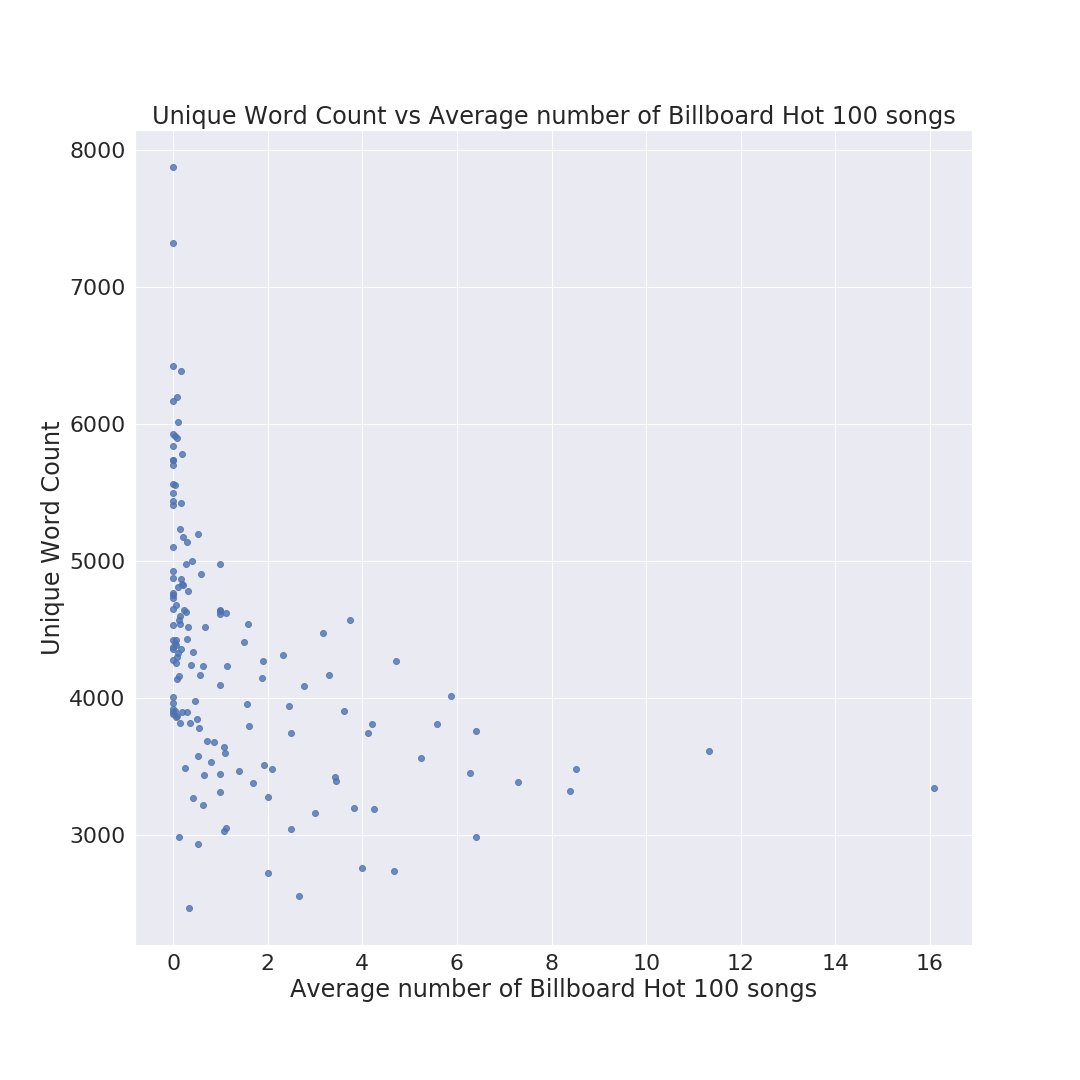
\includegraphics[width=10cm, height=10cm]{./figures/fig1}
	\centering
	\caption{Average number of Billboard 100 songs during artist activity, compared to unique word count across an artists first 35,000 words.}
	\label{fig:fig1}
\end{figure}

\noindent
\newline
To validate the earlier claim that vocabulary range is not indicative of a songwriters ability to write impactful lyrics, the unique word count per artist was compared against the average number of Billboard 100 songs across an artist had across their career. Pearson's Correlation Coefficient , which is used to measure the linear relationship between two variables, was applied to both unique word count and average number of Billboard 100 songs. This resulted in a correlation coefficient of -0.42, indicating a weak inverse correlation between the pairs of data. This value supports the earlier claim that vocabulary range is not indicative of a songwriters ability.

\noindent
\newline
Common methods used to improve songwriting competency include group writing and vocabulary expansion. More recently, software solutions such as MasterWriter(REF) have been used to consolidate previous methods. An inherent problem within software solutions like MasterWriter is the static nature of features such as fixed word and rhyming dictionaries. Consequently, these applications fail to address the ambiguous usage of words resulting from the emerging nature of natural language.

\noindent
\newline
After the completion of song lyrics another secondary problem often faced by less experienced songwriters is choice of instrumental style. 

\section{Goals and Objectives}
\subsection{SONGIFAI - A proposed solution}
The goal of this project is to explore the use of CoVeR derived word embeddings to help with both language modelling and text classification tasks. To contextualise the project aims, both models are applied to a possible use case: a protoype software solution to help reduce common problems faced by songwriters. With this in mind, a prototype solution, SONGIFAI is proposed. SONGIFAI provides two main features namely lyric assistance through predictive text and word suggestions, as well as lyric genre classification. The covariates explored in this project are the following music genres: \textit{Pop}, \textit{Rock} and \textit{Hip-Hop}.
\subsection{High Level Architecture}
\begin{figure}[h]	
	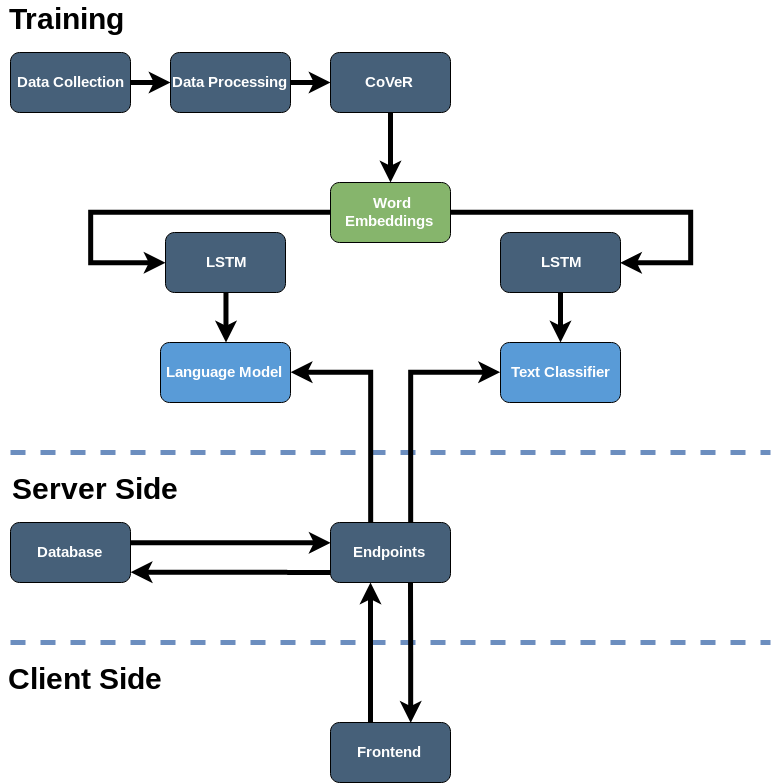
\includegraphics[width=13cm, height=14cm]{./figures/fig7}
	\centering
	\caption{High level architecture for the project}
	\label{fig:fig7}
\end{figure}

 %-----------------------------------------------------
% Chapter: Professional Considerations
%-----
\chapter{Professional Considerations}
\label{prof_con}
Throughout the development of this project both professional and ethical considerations were taken into account, including those highlighted in the British Computing Societies (BCS) Code of Conduct \footnote{https://www.bcs.org/category/6030} and Code of Good Practice. This chapter outlines the relevant areas in the specified documents which have been adhered to during the project.

\section{Code of Conduct}
\subsubsection{Professional Competence and Integrity}
The completion of this project was a large undertaking due to the implementation and integration of a novel machine learning method within a prototype software application. Though the project is beyond the scope of a typical final year project, all work carried out have roots to modules taken in the University of Sussex Computer Science and Artificial Intelligence course, specifically the Neural Networks, Advance Natural Language Engineering and Software Engineering modules. In accordance with section 2.C of the BCS Code of Conduct, background research continually occurred throughout development to maintain a competent standard of professional knowledge.

\subsubsection{Duty of Relevant Authority}
In agreement with section 3.A and 3.B of the BCS Code of Conduct, all scenarios which may cause a conflict of interest between the project and the University of Sussex have been avoided.

\subsubsection{Duty to Professionalism}
In accordance with section 4.A and 4.C of the BCS Code of Conduct, the manner in which this project was conducted was one which maintained the reputation of the BCS. During meetings with other BCS members and professionals such as my project supervisor and work colleagues, appropriate levels of respect and integrity were upheld in accordance with section 4.B of the BCS Code of Conduct.

\section{Good Practices}
The motivation behind this project is one rooted in exploratory research rather than being client driven. Nevertheless, it is important that code produced is well structured and testable to ensure quality assurance. Where possible and in accordance with section 5.2 of the BCS Code of Good Practice, the code produced is well structured and organised to help facilitate further testing and maintainability. 

\noindent
\newline
The same section of the BCS Code of Good Practice refers to the following of programming language guidelines. Both Python and Javascript were used extensively during the development of the project and where appropriate best practices and coding style/conventions have been adhered to. 

\section{Ethical Considerations}
The success of a machine learning project relies heavily on data availability and quality. Regarding song lyrics, there exists no central repository where lyrics, along with the required metadata for the project, are stored. Consequently, a publicly available dataset was used for this project.   

\noindent
\newline
Finally, the project utilises textual data which may have explicit or offensive content within it. After the training of models, which will not be filtered to allow permit artistic freedom, a filtering option will be implemented in order to prevent potential users from seeing unwanted content.
 %-----------------------------------------------------
% Chapter: Related Work
%-----------------------------------------------------
\chapter{Related Work}
\label{chap:related_work}
This chapter briefly outlines previous work relating to the tasks of language modelling and text classification in the area of music lyrics.

\section{Lyric Language Modelling}
Generally, hobbyist approaches to modelling the language used in lyrics have utilized Markov processes, which have the special property that the future is independent of the past given the present. Naturally, as only the present or recent past (in the case of higher order Markov chains) is considered, these types of models are unable to capture longer dependencies and complex structures, such as alliteration and complex rhyme schemes; examples of which are given below:

\begin{figure}[ht]
	\begin{center}
		"Tired of \textbf{injustice}
		\par
		Tired of the \textbf{schemes}
		\par
		Your lies are \textbf{disgusting}
		\par
		What does it \textbf{mean}
		\par
		Kicking me \textbf{down}
		\par
		I gotta get \textbf{up}
		\par
		As jacked as it \textbf{sounds}
		\par
		The whole system \textbf{sucks}"
	\end{center}
	\caption[Example of complex rhyme in Michael Jackson - Scream]{Example of complex rhyme in Michael Jackson - Scream. In this example alternate slant rhymes are used following the \textit{ababcdcd} rhyme scheme.}
\end{figure}

\begin{figure}[ht]
	\begin{center}
		"Hear Her Voice
		\par
		Shake My Window
		\par
		\textbf{S}weet \textbf{S}educing \textbf{S}ighs"
	\end{center}
	\caption[Example of alliteration in Michael Jackson - Human Nature]{Example of alliteration in Michael Jackson - Human Nature. In this example alliteration of the letter S is used in the last line.}
\end{figure}



\noindent
\newline
Recent attempts to model creative writing have utilised neural methods, such as \cite{Zhang2014}, who uses RNN's for Chinese poetry generation and \cite{Potash2015}, who uses an LSTM, to \textit{'ghostwrite'}\footnote{write in the style of X without giving credit} rap lyrics. 

\section{Lyric Genre Classification}
Previous attempts at genre classification predominately use audio features as opposed to lyrics, (in part due to lyric availability). Apart from audio features, the genre of a song is also connected to its lyrics as songs of varying genres use language differently. This can be seen in the Hip Hop, where the use of slang, which are twisted existing words or self-made words (\cite{Edwards2009}) is prevalent. Examples of such words can be seen in \autoref{Tab:Slang}
\begin{table}[ht]
	\centering
	\begin{tabular}{ | p{5cm} | p{5cm} |}
		\hline
		\textbf{Slang Word} & \textbf{Meaning}\\ \hline
		grill & teeth\\ \hline
		lit & fun\\ \hline
		bread & money \\ \hline
	\end{tabular}
	\caption{Example slang words found in the dataset used in the project}
	\label{Tab:Slang}
\end{table}
\newline
Similar to the previous section, genre classification has also been tackled using neural methods. Using audio based features, (\cite{Irvin2016}) and (\cite{Pui2018}), utilise LSTM's for classification. In relation to song lyrics \cite{Tsaptsinos2017} utilises lyrics to train a Hierarchical Attention Network (\cite{Yang2016}), which provide state of the art results for document classification due to their ability to encode its knowledge about the composites of a document in a hierarchical way. In the same paper, a baseline LSTM is implemented for comparative reasons. 
 %-----------------------------------------------------
% Chapter: Background 
%-----------------------------------------------------
\chapter{Background}
\label{chap:background}
This chapter provides an introduction to the theory and previous work within the areas of word embeddings, neural language models and text classification. 

\section{Word Embeddings}
Word embeddings are vectors of predefined size which aim to encode a distributional numerical representation of word features. Recent aforementioned methods of learning these representations include the GloVe, word2Vec and fastText (\cite{Bojanowski2017}) algorithms. The utilization of word embeddings has been highly successful in many natural language processing tasks such as sentiment analysis (\cite{Socher2013}) and syntactic parsing (\cite{Socher2013}). Previous techniques for creating such representations can be categorised into two categories: matrix factorization methods and shallow window-based methods.
\subsection{Previous Methods}
\subsubsection{Global Matrix Factorization Methods}
Global matrix factorization methods such as Latent Semantic Analysis (LSA) use low rank approximations to decompose large matrices containing corpus statistics. Typically these matrices take the form of a term-document matrix, which captures the frequencies of terms across a collection of documents, or a term-term matrix, which store co-occurrence counts of terms. Matrix factorisation methods such as LSA allow for fast training and perform well on word similarity tasks by leveraging word occurrence statistics however they suffer from the disproportionate importance given to large word counts.
\subsubsection{Shallow Window-Based Methods}
Shallow window-based methods provide an alternative approach to learning word representations by sliding a fixed window over the contents of a corpus and learning to predict either the surroundings of a given word (skip-gram model) or predict a word given its surroundings (continuous bag of words). In the case of shallow window-based methods, they are good at capturing more complex patterns and do well in the word analogy task, however they fail to leverage global statistical information such as those used in global matrix factorization methods.
\subsection{GloVe}
Global Vectors for Word Representation (GloVe), is an unsupervised word embedding algorithm, introduced by Pennington et al, which marries the benefits of both global matrix factorisation and shallow window-based methods. Presented as a log-bilinear regression model, GloVe makes use of a global word co-occurrence statistics from a corpus. As detailed in the paper, GloVe outperformed previous methods such as word2vec in word analogy, word similarity and named entity recognition tasks. Conceptually, GloVe is based on the idea that ratios of probabilities of words co-occurring have the potential to encode meaning which is encoded as vector differences. This concept is formalised in the following equation, where the dot product of focal and context word vectors, \(w\) and \(\tilde{w}\), is equal to the logarithm of the probability of the words co-occurring, \(\log{X_{ij}}\).

\begin{equation}
w_{i}^{T} \tilde{w_{j}} + b_{i} + \tilde{b}_{j} = \log{X_{ij}}^{2}
\end{equation}

\noindent
\newline
A weighting function \(f(X_{ij})\) is used to decrease noise caused by very frequent word co-occurrences. The following weighting function is used in the GloVe model.

\begin{equation}
	f(x) =
	\begin{cases}
	(x/x_{max}), & \text{if  \(x <\) } x_{max} \\
	1, & \text{otherwise}
	\end{cases}
\end{equation}

\noindent
\newline
Combining equations 3.1 and 3.2, the GloVe model is defined as a weighted least squares regression problem.
\begin{equation}
	J = \sum_{i, j=1}^{N} f(X_{ij}) (w_{i}^{T} \tilde{w_{j}} + b_{i} + \tilde{b}_{j} - \log{X_{ij}})^{2}
\end{equation}
\subsection{CoVeR - Covariate-Specific Word Embeddings}
Covariates such as author demographics, time and location often accompany documents within a corpus. A trivial approach to obtaining covariate specific word embeddings involves applying GloVe to each subset of corpus documents mapping to a particular covariate. Unfortunately, utilising GloVe this way has certain drawbacks. Firstly, GloVe must be applied individually to sub corpora relating to a specific covariate, which, depending on the number of covariates, is time consuming. As a direct result of this, global co-occurrence statistics are now split into covariate specific co-occurrence statistics and these are not shared between embeddings, which may cause sub-optimal word representations, especially when sub corpora contain a small amount of co-occurrences for GloVe to leverage. 

\noindent
\newline
A known problem when representing words as dense representations using methods such as GloVe, is interpretability of dimensions. Due to conditional GloVe, producing word embeddings per corpora, relating these embeddings to one another becomes a difficult task. 


\noindent
\newline
Learning Covariate-Specific Vector Representations with Tensor Decompositions (CoVeR), proposed by Tian et al, provides an alternative to the conditional GloVe method which offers a framework to make learned embeddings more interpretable. Being an extension of GloVe, CoVer extends Glove's matrix decomposition of co-occurrence matrices to tensor decomposition of co-occurrence tensors, involving the joint learning of word embeddings and covariate specific transformation matrices which represent the effect of a particular covariate on the base embeddings learned. The CoVeR model is presented below.

\begin{equation}
J = \sum_{i, j=1}^{N} \sum_{k=1}^{M} f(X_{ijk}) ((c_{k} \odot w_{i})^{T} (c_{k} \odot \tilde{w}) + b_{ik} + \tilde{b}_{jk} - \log{X_{ijk}})^{2}
\end{equation}

\noindent
\newline
The introduction of covariate specific weight matrices into the objective function allows the authors to interpret dimensions in the base embeddings learned. 


\section{Language Models}
Formal languages such as programming languages are fully specified with precise syntax and semantics which dictate the usage of all reserved words within a language. Contrarily, natural languages, because of their emerging nature, are unable to be formally specified even with the existence of grammatical rules and structures. Unfortunately, rule based systems suffer from the endless possibilities of language usage outside of grammatical rules which are easily interpretable by humans. Moreover the task of consistently updating rule based systems to accommodate such usage is unfavourable.  

\noindent
\newline
Language modelling (LM) is the task of estimating the probability distribution of various linguistic units such as characters, words and sentences. In recent years, the application of LM  has been essential to many natural language process tasks such as speech to text and text summarization. Language models can be classified into two categories, count-based and continuous-space language models. 

\subsection{Count Based Models}
Count based methods such as statistical language models attempt to learn a probability distribution \(P(w_{1},...,w_{i}) \) over of a sequence of words \(w_{1},...,w_{i}\). An example of a count based method is the n-gram model.

\noindent
\newline
An n-gram is a sequence of \(n\) words. Examples of a two word sequences or bigrams include, \textit{"My name"} and \textit{"is Aubrey"}, whilst examples of three word sequences or trigrams, include sequences of words such as \textit{"Hello my name"} and \textit{"is Aubrey Graham"}. The n-gram model which considers the past \(n-1\) words can be formalised as 

\begin{equation}
	P(w_{i} | w_{1},...,w_{i-1}) \approx P(w_{i} | w_{i-n+1},...,w_{i-1})
\end{equation}

\noindent
\newline
The n-gram model relies on Markov assumptions to model the probability of word sequences \(P(w_{1}....w_{n}) \) as being equal to a limited number of previous words. An inherent problem with the n-gram model is sparsity as some word sequences occur rarely or not at all, even in large text corpora. Using the standard n-gram model would yield too many zero probabilities. To circumvent this, techniques such as back-off and smoothing exist. Another disadvantage of n-gram models is that they rely on exact patterns, meaning they fail to recognise syntactically and semantically similar sentences such as "the cat sat on the mat" and "the dog sat on the mat". N-gram models also suffer from the curse of dimensionality due to increased vocabulary sizes. As a result, limited window sizes are used, causing longer dependencies between words to not be captured.

\subsection{Neural Language Models}
To overcome issues faced by count based models, deep learning methods have been used to create neural language models by simultaneously learning word embeddings and the parameters needed to create a joint probability distribution between the word embeddings. \cite{Bengio2003} proposed a feed forward neural language model to help tackle the problem of data sparsity. Recent state of the art approaches such as \cite{Mikolov2010}, abstract language modelling as a form of sequential data prediction and have implored recurrent neural networks to help encode longer dependencies between sequences of words. The strength of these models comes from their ability to consider several preceding words and thus generalise well.

\noindent
\newline
An overview of generic neural network architectures as well as recurrent neural networks and Long-Short Memory networks are given in the following sections.

\subsubsection{Artificial Neural Networks}
In any neural network architecture, the elementary unit of computation is the artificial neuron which takes inspiration from biological neurons. The artificial neuron receives \(n\) inputs which are each weighted by \(n\) weights and summed together with a bias \(b\). The output \(y\) of a neuron is calculated by passing the weighted sum of the inputs into an activation function \(f\). 

\begin{equation}
	y = \left( \sum_{i=1}^{N} x_{i}w_{i} + b\right)
\end{equation}

\noindent
\newline
Typical activation functions include \textit{Sigmoid}, \textit{Tanh} and \textit{ReLu}. A single layer neural network is defined by \(k\) neurons sharing the same input in the same layer. Single layer neural networks have been proven to be \textit{'universal approximators'} (\cite{Hornik1989}) meaning any continuous function can be approximated using this type of network. The process of stacking layers on top of each other leads to multi-layer neural networks. These types of networks are also known as feed-forward networks. The learnable parameters of these networks are the set of weights and biases for each layer. A feed-forward neural network is trained using gradient descent and its parameters are updated using the \textit{backpropagation} algorithm (\cite{Rumelhart1988}).

\begin{figure}[h]
	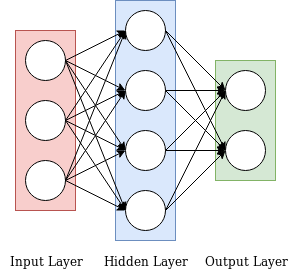
\includegraphics[width=8cm, height=8cm]{./figures/fig2}
	\centering
	\caption{Example neural network, three input nodes, four hidden and two outputs}
	\label{fig:fig2}
\end{figure}

\subsubsection{Recurrent Neural Network}
In a feed-forward neural network, data flow is unidirectional between layers; with data passing through a given neuron at most once. These types of networks perform well on both classification and regression tasks with the assumption that inputs are independent of each other. In tasks dealing with sequential data, feed-forward networks perform poorly. To model sequential data well, a neural network must be able to model the dependencies that exist between successive inputs. The recurrent neural network (RNN) is an attempt to satisfy this requirement by utilising past inputs to help predict future outputs.
\par
\noindent
\newline
In an RNN information is cycled within the network at least once.  An RNN receives a sequence of inputs \(x\) and updates its hidden state \(h_{t}\) by 

\begin{equation}
	h_{t}=
	\begin{cases}
	 0, & \text{t = 0} \\
	 \phi{(h_{t-1}, x_{t})}, & \text{otherwise}
	\end{cases}
\end{equation}

\noindent
where $\phi$ is a nonlinear function such as \textit{tanh} or \textit{ReLu}. The update for the hidden state is usually implemented as 

\begin{equation}
h_{t} = \phi{(Ux_{t} + Wh_{t-1})}
\end{equation}

\noindent
where W and U are weight matrices.

\par
\noindent
\newline
RNN's are trained using gradient descent and backpropagation through time (BBTT), which is identical to performing backpropagation on an \textit{"unrolled"} RNN (seen in figure \autoref{fig:fig3})

\begin{figure}[h]
	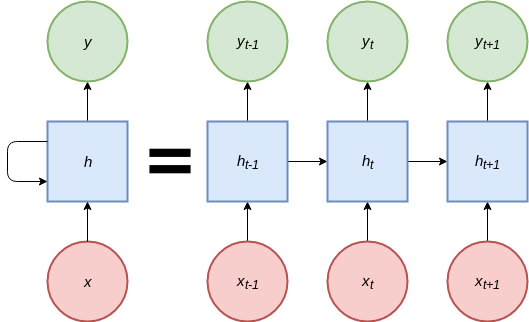
\includegraphics[width=10cm, height=6cm]{./figures/fig3}
	\centering
	\caption{An \textit{unrolled} recurrent neural network can be seen as a feed-forward neural network with many hidden layers}
	\label{fig:fig3}
\end{figure}

\par
\noindent
\newline
During BBTT, back propagation is performed on an unrolled recurrent architecture, causing gradients to back-propagate through numerous network layers. Unfortunately, this has a few major problems. Firstly, a single forward/backward pass through the network is computationally expensive due to the number of hidden layers of the unrolled network being linear to the number of time steps in a sequence. Secondly, this method suffers from the issue of vanishing or exploding gradients(REF) where gradients can decay or grow exponentially as they propagate over time, which can prevent the network from learning entirely.

\subsubsection{Long Short-Term Memory}
Long Short-Term Memory (LSTM) (\cite{Hochreiter1997}) is a variant of the recurrent neural network which is capable of capturing longer dependencies between sequences of data without suffering from vanishing gradients. This is achieved through a feature known as gating; a mechanism which acts as a permissive or restrictive barrier to information flow. 

\noindent
\newline
The core component of the LSTM is the cell state which is able to propagate \textbf{relevant} information throughout the network. This is achieved within the memory cell through the forget, input and output gate. The forget gate regulates how much of the existing memory should be forgotten, the input gate regulates how much of the new cell state to keep, and the output gate regulates how much of the cell state should be allowed into the next layer of the network.

\begin{figure}[h]
	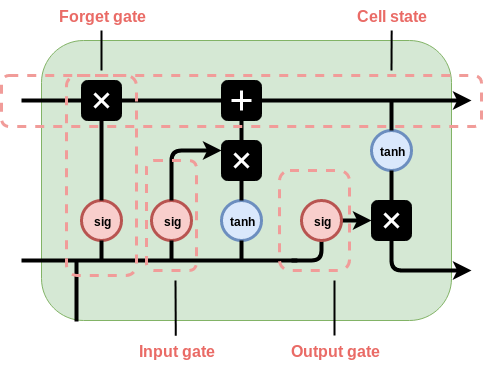
\includegraphics[width=10cm, height=8cm]{./figures/fig4}
	\centering
	\caption{LSTM memory cell, with forget, input and output gates}
	\label{fig:fig4}
\end{figure}

\subsection{Text Classification}
Text classification is a supervised NLP task which involves assigning pre-defined labels to text according to its content. Automated classification of text can be achieved through rule based and machine learning based systems. Rule based methods tackle classification through the use of handcrafted linguistic rules, which assign patterns in text to predefined categories. For example, given two word lists which  Rule based systems don't come without drawbacks, firstly to create such a system requires deep domain knowledge. Moreover, unlike the previous example, creating, maintaining and scaling such rules is challenging and time consuming. 
\subsubsection{Traditional Methods}
Before a classifier can be trained, textual inputs must be transformed into numerical representations in a process known as feature extraction. A common method for feature extraction is the bag of words approach which given a vocabulary set \(V\), creates an input vector which represents word counts for each word of the vocabulary. For example, if we define the vocabulary \(V\) ..

\noindent
\newline
Two common classifiers, namely Naive Bayes classifiers and support vector machines are outlined below

\paragraph{Naive Bayes}
\noindent
\newline 
Naive Bayes Classification is a generative approach which uses bayes theorom to learn a join probability distribution .... Naive bayes classification is a robust method for training a text classifier which can achieve accurate results without large amounts of training data.

Naive bayes is a classification techinque based on bayes theroem with an assumpoion of inde[endence among preictors. A naives bayes c;assifier assumes that the precence of a particular fgeature in a class is unrelsted tp the [recence of any other fetaure.

\paragraph{Support Vector Machines}
\noindent
\newline 
A Support Vector Machines (SVM) (Vapnik et al 1995) is a discriminative classifier that aims to find a linear classification boundary or \textit{hyperplane} to discriminate between classes in high dimensional space. SVM's achieve this through support vectors, random training data points, which are used to maximise the margin between ... Similar to naive bayes classifiers, SVM's do not require large amounts of training data to achieve accurate results. SVM's were introduced to the problem of text classification by Joachims(REF)

\subsubsection{Deep Learning Methods}
 %-----------------------------------------------------
% Chapter: Requirements Analysis
%-----------------------------------------------------
\chapter{Requirements Analysis}
\label{chap:requirements_analysis}
As the project involves the development of a prototype software system, it is important to consider the project from a software engineering perspective. Moreover, the project involves the integration of a novel machine learning model, with the success of the project relying heavily on factors such as data availability, data quality and processing power. With this and other considerations such as training time and implementation complexity in mind, it is necessary to define software requirements in order to constrain the project goal to one that is achievable. Software requirements should also be inferred from the needs of the end-user and as such it is necessary to understand user needs through existing solutions. This chapter briefly evaluates two existing solutions and outlines the functional and non-functional requirements by which the prototype will be evaluated.
\section{Existing Solutions}
\subsection{MasterWriter}
Self-described as "The most powerful suite of writing tools ever assembled in one program.",
MasterWriter 5 is a software application which aims to help songwriters, poets and creative
writers with their works. Available as a desktop, mobile or tablet application, it consolidates a
number of writing tools into one application. These tools are outlined in the table below:


\subsection{Rhymer's Block}
Rhymer's block is a mobile application intended to help writers specifically with rhymes. Providing real time rhyme suggestions, the application allows users to quickly write lyrics and provides a social feature in order to share lyrics and review lyrics from other users.

\subsection{Evaluation of existing solutions}
A common feature to both software solutions is that of word suggestion, specifically suggestion of rhyming words. Furthermore both solutions provide functionality for users to write, edit and save lyrics within the application.
\section{Requirements}
In this section the requirements for the project will be set out. The functional requirements will specify what the software will do whilst the non-functional requirements will detail how these will be done.

\subsection{Functional}
\begin{table}[ht]
	\caption{SONGIFAI Functional Requirements}
	\centering
	\begin{tabular}{ | l | p{10cm} | l | }
		\hline
		\textbf{ID} & \textbf{Description} & \textbf{Dependency} \\ \hline
		FR1 & The system should allow users to input lyrics & N/A \\ \hline
		FR2 & The system should allow users to load/save lyrics & N/A  \\ \hline
		FR3 & The system should be able to classify user submitted lyrics as either Pop/Rock/Hip Hop & N/A \\ \hline
		FR4 & The system should be be able to suggest words from a given word. These words should be the most similar words in the covariate word embedding space & N/A \\ \hline
		FR5 & The system should be able to provide real time text prediction whilst a user is in edit mode & N/A \\ \hline
		FR6 & The system should allow for the filtering of explicit content in both the word suggestion and word prediction feature & N/A \\ \hline
		FR7 & The user should be able to change the underlying covariate specific word embeddings used or the base embeddings if required & N/A \\ \hline
		FR8 & 10C & N/A \\ \hline
	\end{tabular}
	\label{Tab:Tcru}
\end{table}
\subsection{Non-Functional}
\begin{table}[ht]
\caption{SONGIFAI Non-Functional Requirements}
\centering
	\begin{tabular}{ | l | p{10cm} | l | }
		\hline
		\textbf{ID} & \textbf{Description} & \textbf{Dependency} \\ \hline
		NFR1 & The system should take the form of a web application and be able to be rendered on different device types & N/A \\ \hline
		NFR2 & The word prediction process should return a list of candidate words in real time & N/A \\ \hline
		NFR3 & 10C & N/A \\ \hline
	\end{tabular}
	\label{Tab:Tcr}
\end{table}



 %-----------------------------------------------------
% Chapter: Methodology
%-----------------------------------------------------
\chapter{Methodology}
This chapter describes the methodology used during this project. 
\label{chap:data_methodology}
\section{Collecting Data}
As previously mentioned, a central repository for song lyrics, where downloading is permissive, is non-existent. Collection of song lyrics from sites such as Genius\footnote{https://genius.com/} is only achievable through web scraping: a process which involves the exhaustive downloading and processing of web pages from either a predefined list of URLs or the recursive process of link extraction and following (commonly known as \textit{web crawling}) from a given seed URL. When scraping at scale, restrictions such as the robots exclusion protocol, which specifies areas of a website that are allowed to be processed, and crawl rate, which specifies the minimum delay between requests, make data collection a troublesome task. Taking into account the project aims and constraints such as time, web scraping was deemed unfavourable and hence avoided for data collection.

\noindent
\newline
To fulfil the data requirements of the project, a public dataset \footnote{https://www.kaggle.com/neisse/scrapped-lyrics-from-6-genres} containing over 250,000 song lyrics was used. The dataset, which was scraped from Brazilian music website Vagalume, comprised of two \textit{.csv} files: artists-data and lyrics-data. The artist-data file included metrics such as popularity, genre and number of songs per artist, whilst the lyrics-data file contained song lyrics for individual songs by artists.

\section{Data Analysis and Restructuring}
The CoVeR algorithm requires each document within a corpus to be associated with a covariate in order to jointly learn word embeddings and the relevant transformation matrices. To satisfy this requirement, Pandas, a Python data analysis library, was used to perform a join operation on the artists columns in both the artists-data and lyrics-data files. The result of this operation followed by the additional dropping of redundant columns resulted in the dataset used throughout the rest of the project.

\noindent
\newline
(IMAGE OF DATASET SCHEMA)

\noindent
\newline
A trivial approach to split the lyric corpora on genre would involve an equal split for equal representation, however, this method uses the assumption that for each genre, word count per song is equivalent. Examining the dataset however, proved this not to be the case.
\begin{figure}[h]
	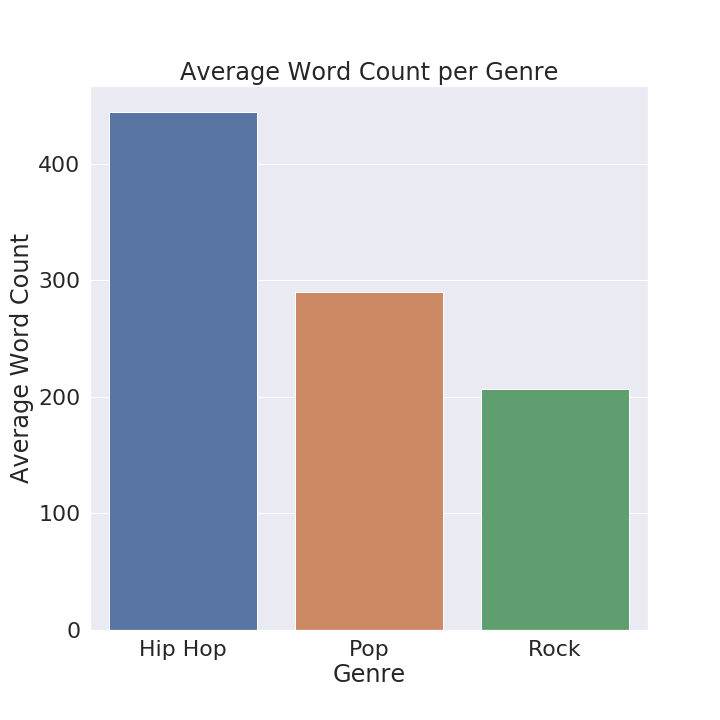
\includegraphics[width=8cm, height=8cm]{./figures/fig6}
	\centering
	\caption{Average word count per lyric per genre in the dataset}
	\label{fig:fig6}
\end{figure}

\noindent
\newline
Analysing the dataset, the mean number of words contained in a hip hop song was 444; being more than double the mean number of words found in rock songs which had a count of 207. With regards to pop, the mean word count per song was 289. To reflect these statistics and also due to constraints in the distribution of data by genre, 100,000 song lyrics were randomly selected to create the dataset to be used to train CoVeR. Moreover a data split of 48:30:22 for Rock, Pop and Hip-Hop, was to maintain an even distribution of words by song genre within the dataset.
\section{Data Pre-processing}
Essential to any machine learning task is the pre-processing of input data in such a way that important features are accessible during training. In natural language processing, this can include techniques such as tokenisation, string cleaning, stemming and lemmatisation.

\noindent
\newline
Following data reconstruction, each song lyric in the dataset was cleansed and tokenised. The following string cleaning techniques were applied to each song lyric.

\begin{enumerate}
	\item All letters were lowercased.
	\item All characters, except for letters, were substituted with a space.
	\item All text between brackets were removed. (This was to ensure text like \textbf{[Verse 1]} was not included during training).
	\item All trailing white space was removed.
\end{enumerate}

\noindent
\newline
Tokenisation is the process of separating textual inputs into meaningful chunks called \textit{tokens}. Naturally to create word embeddings, text is tokenised at the word level and each token is assigned a unique integer key to map the token to its future word embedding.

\section{Hyperparameters}
In machine learning hyperparameters are parameters that govern a given model. The selection of these parameters directly impacts the performance of a given training algorithm and as such, hyperparameter choice is important for producing optimal performance for a given model. Both CoVeR and LSTM networks have important hyperparameters which are reviewed in the following sections.
\subsection{CoVeR Hyperparamters}
\subsubsection{Removing Rare Words}
Word embedding methods such as word2vec typically remove rare occurring words within a corpus before training takes place. In the case of word2vec, rare words are removed, \textit{before} the computation of co-occurrence statistics. This method of removal has the effect of generating  context windows differing to the context windows generated from the original corpus. In turn this produces differing \(i,j\) co-occurrences. This is highlighted in the example below.

\noindent
\newline
Sentence: Fly me to the moon.
\noindent
\newline
Context of "to" (without removal of rare words): me, the
\noindent
\newline
Context of "to" (with removal of rare words): Fly, moon

\noindent
\newline
Neither the CoVeR or GloVe paper, discuss the removal of rare words, however many implementations (REF) 
\subsubsection{Subsampling}
Typically found within text corpora are high frequency stop words which provide less information than rarely occurring words (\cite{Mikolov2013a}). For example This concept can also be applied to word embeddings; where the word embeddings of frequent words does not change significantly after training on several examples. Taking inspiration from word2vec, subsampling was used at the covariate level using the following adapted formula from the original word2vec implementation.

\begin{equation}
P(w_{ik}) = \sqrt{\dfrac{z(w_{ik})}{t}} + 1 \cdot \dfrac{t}{z(w_{ik})}
\end{equation}

\noindent
\newline
where \(z(w_{ik})\) is the percentage of word \(w_{ik}\) in covariate \(k\) and \(t\) is a chosen threshold.
\subsubsection{Context Windows}
CoVeR uses the same weighted context windows strategy as GloVe during the process of calculating co-occurrence statistics. The CoVeR paper uses a context window size of 8, however the paper does not specify whether they used symmetric or asymmetric windows during their experiments. As such, both are experimented with whilst performing hyperparameter tuning.  
\subsubsection{Embedding Size}
\subsubsection{Optimiser}
\subsubsection{Tuning}
\subsection{LSTM Hyperparameters}
\subsubsection{Dropout}
Dropout is a regularization technique proposed by \cite{Srivastava2014}, which involves the random dropping of nodes and their connections within a network. Selected nodes are picked at random using a probability known as the dropout rate. Dropout helps to decrease over-fitting as 
\subsubsection{Embedding Layer}
\subsubsection{Optimiser}


 %-----------------------------------------------------
% Chapter: Prototype Implementation
%-----------------------------------------------------
\chapter{Implementation}
\label{chap:implementation}
Implementation of the project predominately utilised the  Python\footnote{https://www.python.org/} programming language. The motivation for using Python originated from prior familiarity with the language, and it's collection of machine learning and web development libraries which form two key components of the project. Though Python allows for relatively quick development, its known drawback of speed was a cause of concern.

\noindent
\newline
As stated in \autoref{chap:requirements_analysis}, in research, model training time is often neglected in favour of high performing models. As this project involves the creation of a prototype software application, it was important that the impact of model training time on overall development was minimal.

\noindent
\newline
This chapter describes the development process for implementing the CoVeR algorithm, the language and text classification models as well as the SONGIFAI web application. 

\section{Hardware Specification}
All implementation was completed on a personal machine. The hardware specifications for the machine are highlighted below

\begin{table}[h!]
	\centering
	\begin{tabular}{||c | c||} 
		\hline
		Hardware Component & Specification \\ [0.5ex] 
		\hline\hline
		CPU & Intel Core i7-8750H CPU @ 2.20GHz x 12 \\ 
		GPU & NVIDIA GeForce GTX 1050 Ti 4GB \\
		RAM & 16GB \\
		\hline
	\end{tabular}
	\caption[Hardware Specification]{Hardware specification for machine used throughout development}
	\label{table:1}
\end{table}
\section{Calculating Co-occurrence Statistics}
Many unsupervised NLP methods compute co-occurrence statistics before learning takes place. Typically, co-occurrence statistics, such as GloVe's word-word co-occurrence matrix contain sparse data, and computing them can often be a computationally more expensive task than the learning itself. The original GloVe paper describes this process as a \textit{'one-time upfront cost'}, with the assumption that selected corpora are static. Unfortunately, for many NLP pipelines such corpora are more dynamic in nature. For example, social data from online platforms such as Twitter\footnote{https://twitter.com/} are in constant flux and relying on pre-computed co-occurrence statistics to learn Twitter based word embeddings is sub-optimal. Compared to GloVe, computing the co-occurrence statistics for CoVeR has added complexity due to the transition from a co-occurrence matrix to a co-occurrence tensor.

\noindent
\newline
Attempts to efficiently compute co-occurrence counts include the usage of distributed computing techniques such as \textit{MapReduce} (\cite{Lin2008}, \cite{Wittek2013}). MapReduce is a model for distributed computing which at its crux involves two functional processes: \textit{map} and \textit{reduce}. During the map process, data is taken in as key/value pairs and transformed into intermediary key/value pairs. These are then passed to the reduce process which aggregates data which share the same key. An example MapReduce process is walked through in \autoref{fig:fig14} below. 

\begin{figure}[h]
	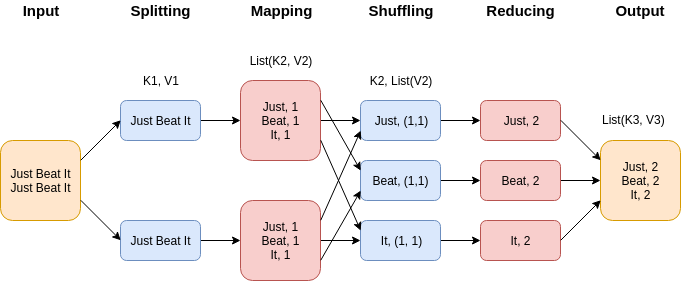
\includegraphics[width=14cm, height=6cm]{./figures/fig14}
	\centering
	\caption[MapReduce Word Count Example]{MapReduce word count example:}
	\label{fig:fig14}
\end{figure}
\noindent
Apache Spark is an open-source framework, written in Scala, for distributed computing and has recently emerged as the de-facto choice for big data processing over Apache Hadoop. Like Hadoop, Spark also supports the MapReduce programming paradigm but boasts features such as enhanced speed, a distributed data structure, as well as API's written in multiple programming languages. Spark uses a master/slave architecture to achieve distributed computing. The \textit{driver} acts as the master node and distributes tasks to many different worker nodes, also known as \textit{executors}, which each run their own JVM processes to execute tasks.

\begin{figure}[h]
	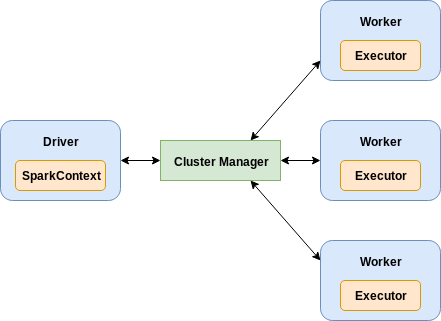
\includegraphics[width=8cm, height=5cm]{./figures/fig19}
	\centering
	\caption{High level view of the Spark Architecture. The spark context is where the main program is defined, which is then split into tasks to be completed via numerous executors.}
	\label{fig:fig19}
\end{figure}

\noindent
\newline
PySpark, a Python API for Spark was initially to pre-process and calculate co-occurrence counts for the dataset. 
Unfortunately, the overhead of collecting completed executor tasks to the driver as well as the cross language communication between Python and Scala made PySpark an unfavourable option for collecting co-occurrence counts. A similar parallelised approach which avoided cross language communication involved the use of Python's multiprocessing module. However this method suffered from Pythons Global Interpreter Lock (GIL) which prevents shared access of Python objects across multiple threads. Taking inspiration from GloVe's original implementation, which is written in C, Cython, an extension of Python, was used to quickly process co-occurrence counts.

\noindent
\newline
Cython is a superset of the Python programming language which aims to provide C like performance whilst maintaining the ability to write Python like code. Native Python programs can experience major speed improvements using Cython because of its ability to compile Python to C code. Ultimately, calculating the co-occurrence statistics for CoVeR was achieved using Cython which provided major speed ups compared to the parallelised approaches outlined before. To highlight these gains, the implementation was compared against its Python equivalent, as well as a commonly used Python implementation of GloVe, developed by Simon Grady\footnote{https://github.com/GradySimon/tensorflow-glove}. This can be seen in \autoref{fig:fig15}.

\begin{figure}[ht]
	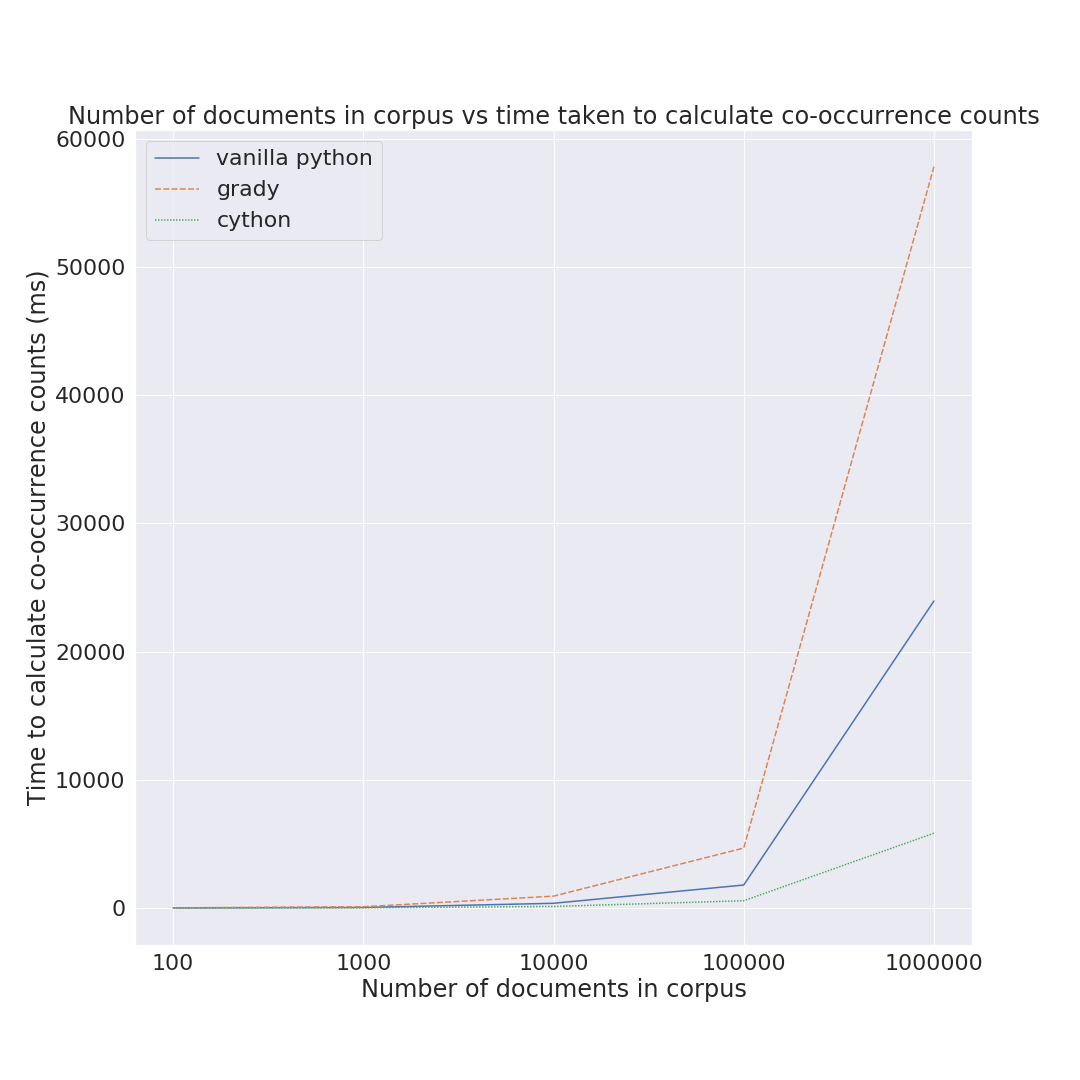
\includegraphics[width=13cm, height=13cm]{./figures/fig15}
	\centering
	\caption[Co-occurrence benchmarks]{A comparison of  }
	\label{fig:fig15}
\end{figure}

\noindent
\newline
\section{CoVeR Implementation}
At time of writing, no public implementation of CoVeR is available. As a result and to meet the needs of this project, CoVeR was implemented using the PyTorch library. PyTorch is a Python library based on Torch, which supports Numpy like operations which can be accelerated through the GPU. The training parameters are highlighted in \autoref{Tab:coverparams} .
\begin{table}[h!]
	\centering
	\begin{tabular}{||c | c||} 
		\hline
		Hyperparameter & Value \\ [0.5ex] 
		\hline\hline
		Embedding Size & 50 \\ 
		Window Size & 8 \\
		Batch Size & 512 \\
		Epochs & 10 \\
		Optimiser & Adam \\
		Subsample Threshold & 0.05 \\
		\hline
	\end{tabular}
	\label{Tab:coverparams}
	\caption[CoVeR Hyperparameters]{CoVeR Hyperparameters}
\end{table}
\section{Model Implementations}
Implementation of the language models and text classifier was done using Keras. Keras is a high level machine learning library written in Python, which runs on top of either Tensorflow or Theano. The motivation behind using Keras comes from its ease of use to quickly develop deep learning networks. In this project Keras is deployed using Tensorflow as a backend, specifically for its GPU capabilities. As stated in \autoref{chap:data_methodology}, the architectural structure of the language models and the text classifier was the same. From an implementation standpoint differences occurred in the number of hidden units for the LSTM used, as well as the size of the inputs into the network. 



\section{SONGIFAI}
\subsection{Architecture}
SONGIFAI, the prototype system takes the form of a web application. Typically the development of such systems follows the model-view-controller (MVC) paradigm, where the model represents application state, the view presents the state to the user and the controller interfaces between the two. For this prototype, the MVC design pattern was followed. The overall SONGIFAI system architecture can be seen in \autoref{fig:songifaiarc} and screenshots of the application can be found in \autoref{app:screen}.
\begin{figure}[ht]
	\centering
	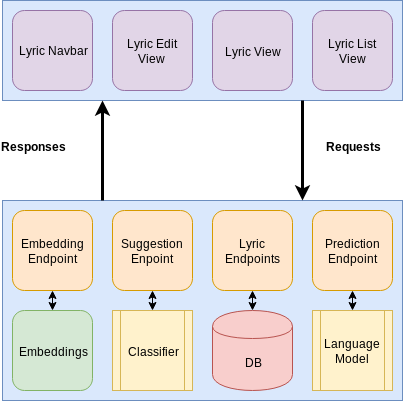
\includegraphics[width=8cm, height=8cm]{./figures/fig22}
	\caption[SONGIFAI Architecture]{SONGIFAI Architecture}
	\label{fig:songifaiarc}
\end{figure}

\subsubsection{Client Side}
For the client side development of SONGIFGAI, requirement NFR1 states that the system must take the form of a web application. However, being a prototype solution, it was important that development was swift and well structured so that the research goals of the project were not hindered. To help achieve this, ReactJS was chosen as the front-end development framework.

\noindent
\newline
ReactJS, (simply known as React) is a JavaScript framework for building user interfaces originally developed and maintained by Facebook. A key concept in React is the idea of components which all React user interfaces are composed off. Simply put a React component takes properties as input and outputs a UI using those properties. Comparable to the object oriented programming paradigm, React promotes the reuse of code through high modularized components.

\subsubsection{Server Side}
Requirement FR1 refers to a user of the system being able to save, load and edit their lyrics. Moreover for easy compatibility with Keras generated models, another Python based library was used for server side development. Django is a python based web framework which follows the model-view-template (MVT) architectural pattern(REF), although for this project it was adapted to the MVC pattern due to the user interface being handled by React. Out the box, Django comes with a configured database, an administration panel, and simple mechanism to create restful endpoints. These were very favourable for the swift development of the prototype system.

\noindent
\newline
Both the client and server were developed in Docker containers, which allow for easy deployment to hosted services. As this was a prototype application, actual deployment was not considered, though the mechanisms are in place for easy future deployment. 
 %-----------------------------------------------------
% Chapter: Evaluation
%-----------------------------------------------------
\chapter{Evaluation}
\label{chap:evaluation}
\section{CoVeR Evaluation}
\subsection{Validating Implementation}
\subsubsection{Base Embeddings}
As previously stated, there currently does not exist any public implementation of the CoVeR algorithm. As a basis for validating the quality of the CoVeR model created in this project, the base embeddings generated were compared against embeddings generated using the Glove algorithm. In order to achieve this, a simple framework was set up to compare the the most similar words for each word in both the CoVeR and GloVe embeddings. For this experiment, each model was generated by using a symmetric context window of size 8 and each had a dimensionality of 50. Staying true to both papers, the Adam optimiser was used to train the CoVeR algorithm, whilst the AdaGrad optimiser was used to train GloVe. Both models were trained for 10 epochs. 

\noindent
\newline
To find the most similar words for a given word in both the CoVeR and GloVe model, the cosine similarity measure was used.

\begin{equation}
sim(A, B) =\dfrac{A \cdot B}{\lVert A \rVert \lVert B \rVert}
\end{equation}



\subsubsection{Covariate Specific Embeddings}
The original CoVeR paper validates the quality of the learned covariate weight matrices by clustering. This was done 
\section{Model Evaluations}
\subsection{Language Model}
Typically, language models can be evaluated using either extrinsic or intrinsic methods. Whilst extrinsic evaluation methods measure the performance of a model when applied to an application, intrinsic methods allow for the evaluation of a model independent of any application. A drawback of using extrinsic evaluation is the that it is computationally expensive, as it involves the the full deployment of an application to a task, which then has to be evaluated using 
\subsubsection{Intrinsic Evaluation}
A typical intrinsic evaluation metric used to evaluate a language model is perplexity(REF 19, 30, 43). Perplexity is a measure of how well a given language model will predict test data. The general formula for perplexity is given below

\noindent
\newline
From this 

\begin{figure}[h]
	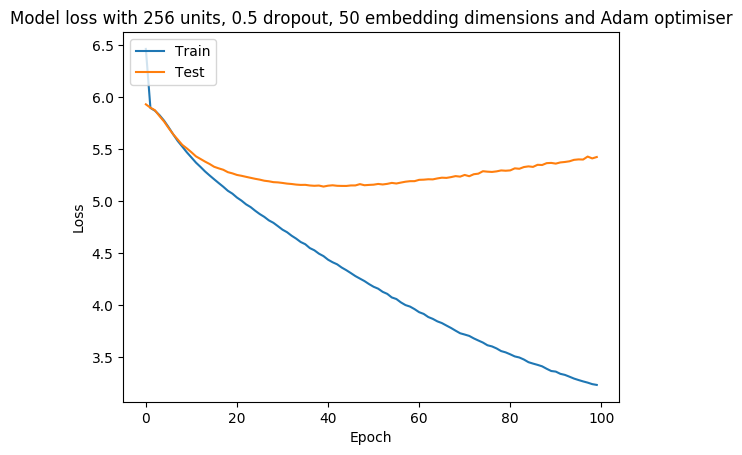
\includegraphics[width=9cm, height=6cm]{./figures/poploss}
	\centering
	\caption{poploss}
	\label{fig:poploss}
\end{figure}

\begin{figure}[h]
	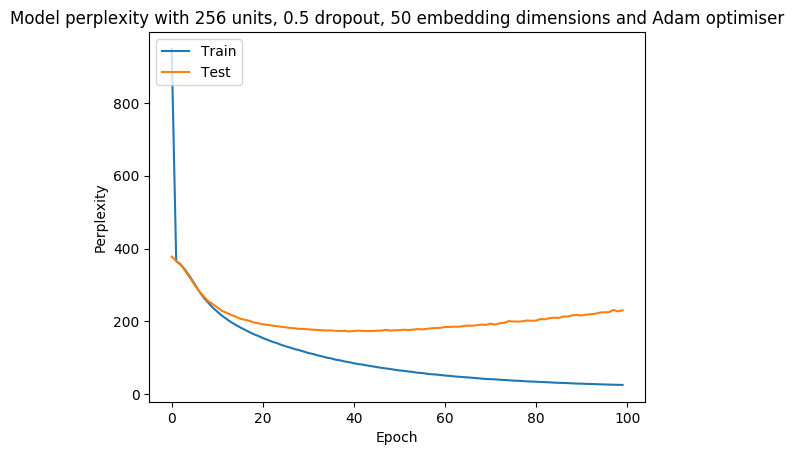
\includegraphics[width=9cm, height=6cm]{./figures/popper}
	\centering
	\caption{popper}
	\label{fig:popper}
\end{figure}

\begin{figure}[h]
	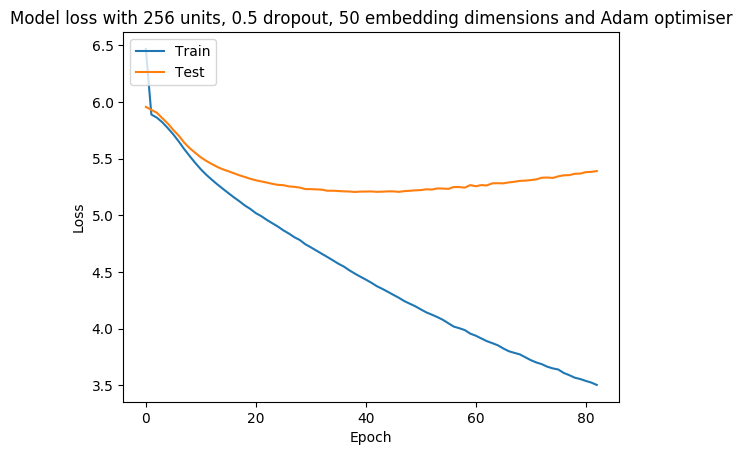
\includegraphics[width=9cm, height=6cm]{./figures/rockloss}
	\centering
	\caption{rockloss.}
	\label{fig:poploss}
\end{figure}

\begin{figure}[h]
	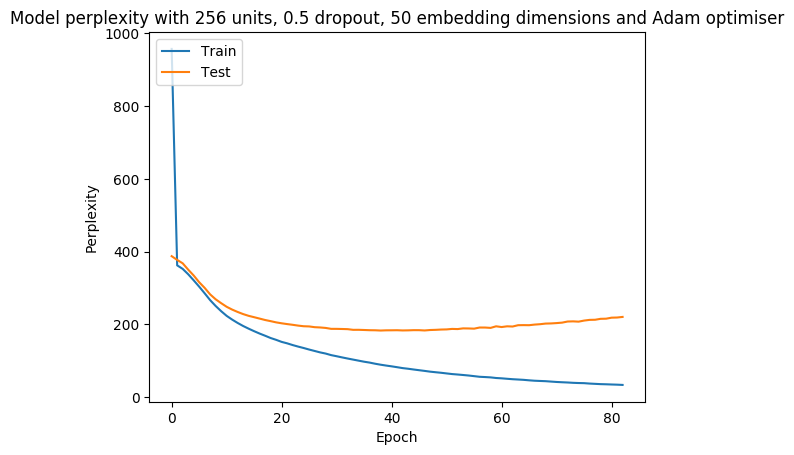
\includegraphics[width=9cm, height=6cm]{./figures/rockper}
	\centering
	\caption{rockper.}
	\label{fig:popper}
\end{figure}

\begin{figure}[h]
	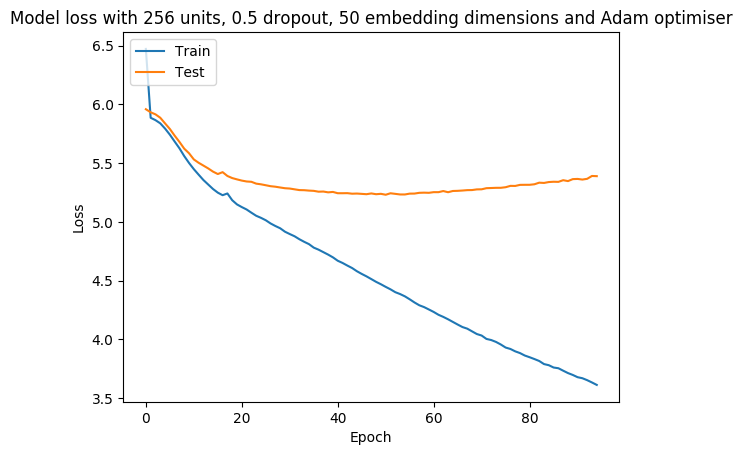
\includegraphics[width=9cm, height=6cm]{./figures/hiphoploss}
	\centering
	\caption{hiphoploss}
	\label{fig:poploss}
\end{figure}

\begin{figure}[h]
	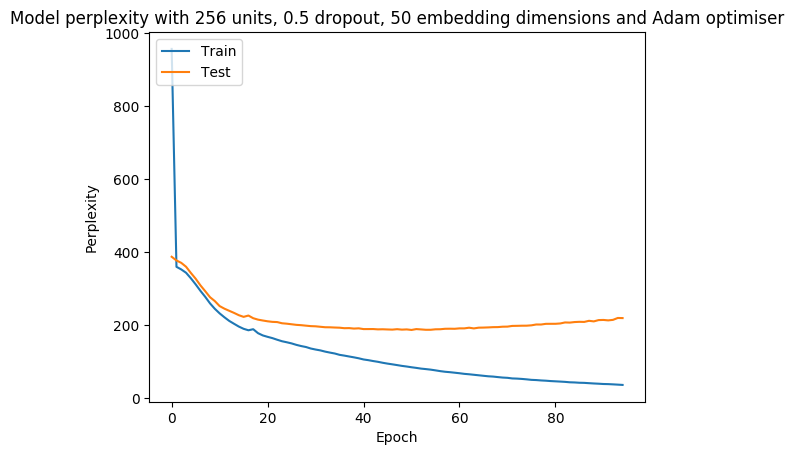
\includegraphics[width=9cm, height=6cm]{./figures/hiphopper}
	\centering
	\caption{hiphopper}
	\label{fig:popper}
\end{figure}

\noindent
\newline


\subsection{Text Classification}
In order to further evaluate the covariate specific word embeddings produced by CoVeR, each covariate embedding was used to train a binary classifier that would discriminate lyrics as either belonging to that particular covariate or not. These were compared with GloVe trained word embeddings to see if the the covaraiets specific word embeddings did indeed capture the semantics of the genre better than generic glove embeddings. The results of the test can be seen in ... below

\begin{table}[ht]
	\centering
	\begin{tabular}{ | p{3cm} | p{2cm} | p{2cm} | p{2cm} | p{2cm} |}
		\hline
		\textbf{Embedding} & \textbf{Training Loss} & \textbf{Training Accuracy} & \textbf{Validation Loss} & \textbf{Validation Accuracy}\\ \hline
		GloVe & 0.5807 & 0.6906 & 0.6194 & 0.6698\\ \hline
		Pop Covariate & 0.5791 & 0.6925 & 0.6122 & 0.6730\\ \hline
	\end{tabular}
	\label{Tab:GlovePopClass}
	\caption{GlovePopClass}
\end{table}

\begin{table}[ht]
	\centering
	\begin{tabular}{ | p{3cm} | p{2cm} | p{2cm} | p{2cm} | p{2cm} |}
		\hline
		\textbf{Embedding} & \textbf{Training Loss} & \textbf{Training Accuracy} & \textbf{Validation Loss} & \textbf{Validation Accuracy}\\ \hline
		GloVe & 0.5251 & 0.7238 & 0.5691 & 0.6985\\ \hline
		Rock Covariate & 0.5200 & 0.7260 & 0.5646 & 0.7009\\ \hline
	\end{tabular}
	\label{Tab:GloveRockClass}
	\caption{GloveRockClass}
\end{table}

\begin{table}[ht]
	\centering
	\begin{tabular}{ | p{3cm} | p{2cm} | p{2cm} | p{2cm} | p{2cm} |}
		\hline
		\textbf{Embedding} & \textbf{Training Loss} & \textbf{Training Accuracy} & \textbf{Validation Loss} & \textbf{Validation Accuracy}\\ \hline
		GloVe & 0.4511 & 0.7926 & 0.5115 & 0.7760\\ \hline
		Hip Hop Covariate & 0.4593 & 0.7878 & 0.4985 & 0.7823\\ \hline
	\end{tabular}
	\label{Tab:GloveHipHopClass}
	\caption{GloveHipHopClass}
\end{table}
\section{SONGIFAI}
\subsection{Requirements Evaluation}

 %-----------------------------------------------------
% Chapter: Conclusion
%-----------------------------------------------------
\chapter{Conclusion}
\label{chap:conc}

I was right all along.

\section{What was I right about?}

I was right about the following things.

\subsection{Previous theories were wrong}

People thought they understood, but they didn't.

\subsection{My new idea is right}

Of course.

%%%%%%%%%%%%%%%%%%%%%%%%%%%%
% BIBLIOGRAPHY
\clearpage
\phantomsection
\addcontentsline{toc}{chapter}{Bibliography}
\bibliography{bib}
%%%%%%%%%%%%%%%%%%%%%%%%%%%%


%%%%%%%%%%%%%%%%%%%%%%%%%%%%
% START APPENDICES
\appendix
%%%%%%%%%%%%%%%%%%%%%%%%%%%%


%-----------------------------------------------------
% Appendix: Code
%-----------------------------------------------------
\chapter{Language Model Perplexities}
\label{app:code}
\begin{figure}[ht]
	\centering
	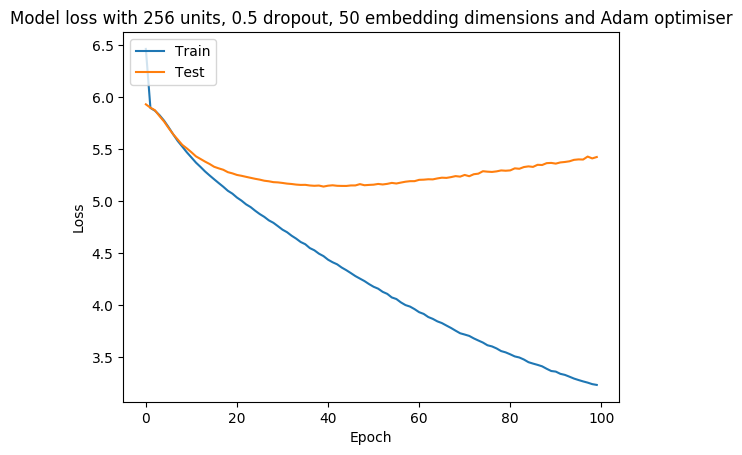
\includegraphics[width=11cm, height=7.5cm]{./figures/poploss}
	\caption{Pop Language Model Loss}
	\label{fig:poploss}
	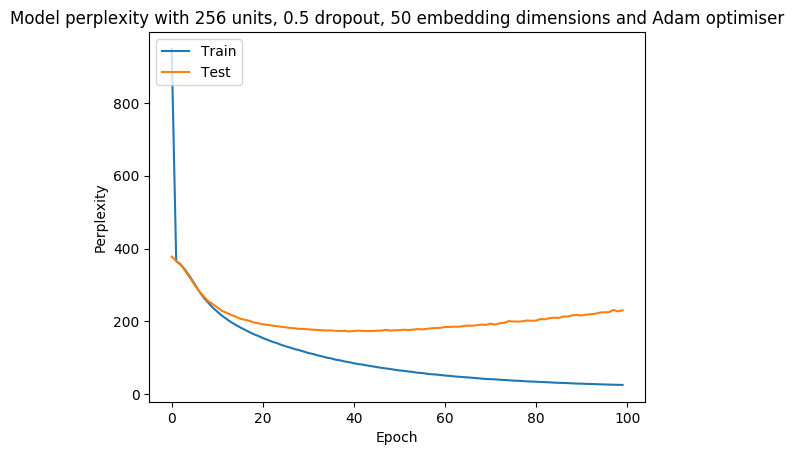
\includegraphics[width=11cm, height=7.5cm]{./figures/popper}
	\caption{Pop Language Model Perplexity}
	\label{fig:popper}
\end{figure}

\begin{figure}[ht]
	\centering
	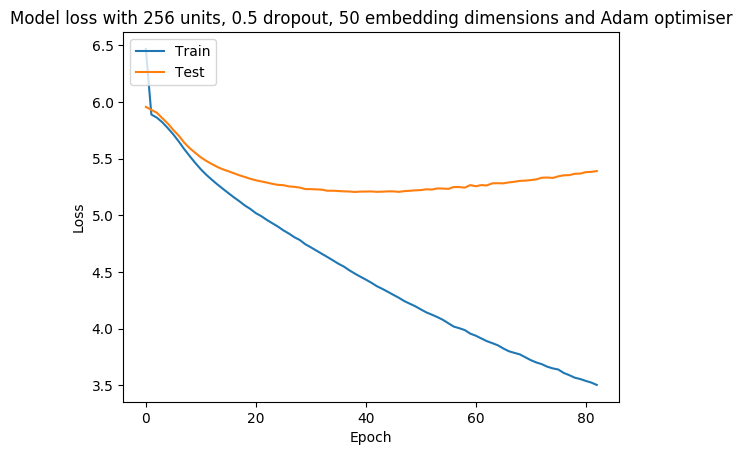
\includegraphics[width=11cm, height=7.5cm]{./figures/rockloss}
	\caption{Rock Language Model Loss}
	\label{fig:poploss}

	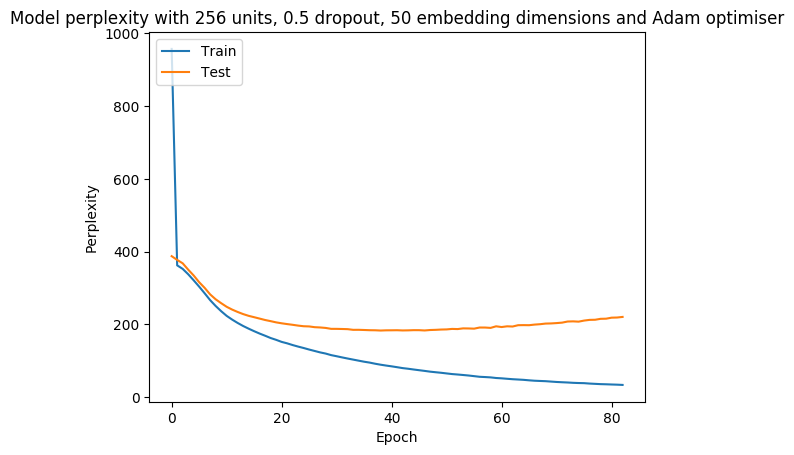
\includegraphics[width=11cm, height=7.5cm]{./figures/rockper}
	\caption{Rock Language Model Perplexity}
	\label{fig:popper}
\end{figure}

\begin{figure}[ht]
	\centering
	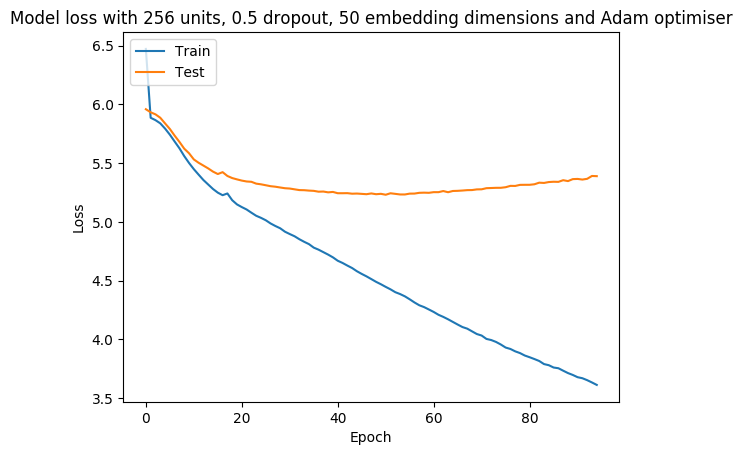
\includegraphics[width=11cm, height=7.5cm]{./figures/hiphoploss}
	\caption{Hip Hop Language Model Loss}
	\label{fig:poploss}
	
	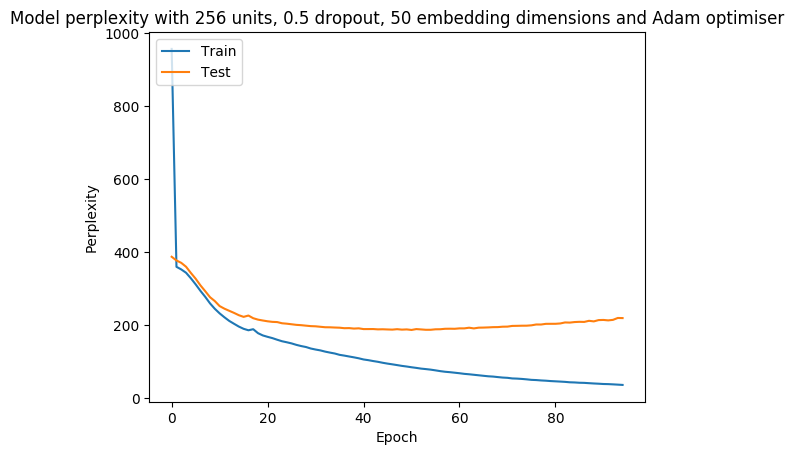
\includegraphics[width=11cm, height=7.5cm]{./figures/hiphopper}
	\caption{Hip Hop Language Model Perplexity}
	\label{fig:popper}
\end{figure}

\chapter{SONGIFAI Screens}
\label{app:screen}
\begin{figure}[h]
	\centering
	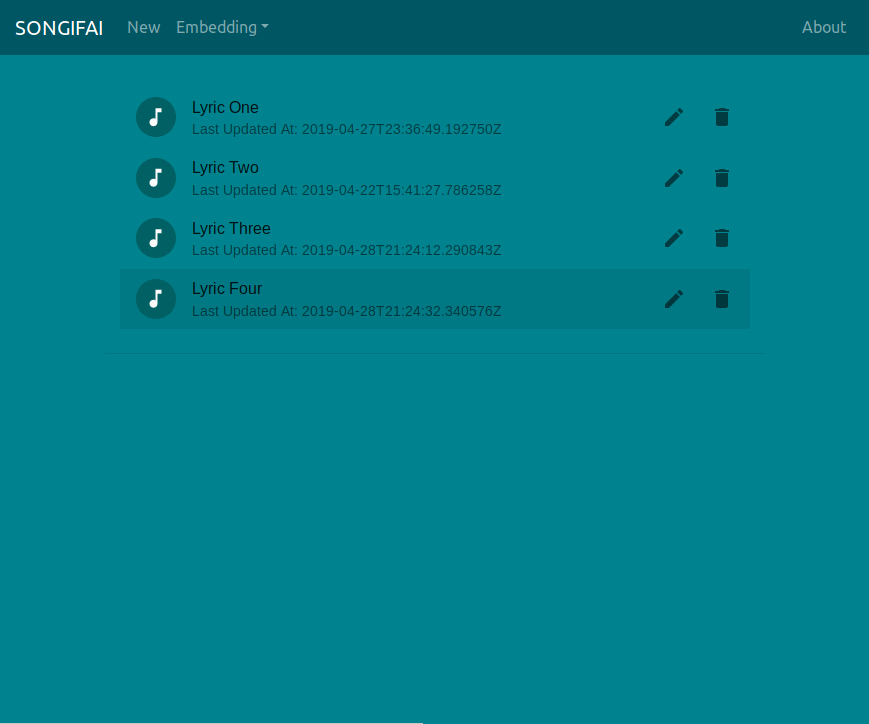
\includegraphics[width=12cm, height=12cm]{./figures/fig20}
	\caption[SONGIFAI Home Page]{SONGIFAI Home Page: Users can see their current list of lyrics and view, edit or delete a selected lyric.}
	\label{fig:songifaihome}
\end{figure}
\begin{figure}
	\centering
	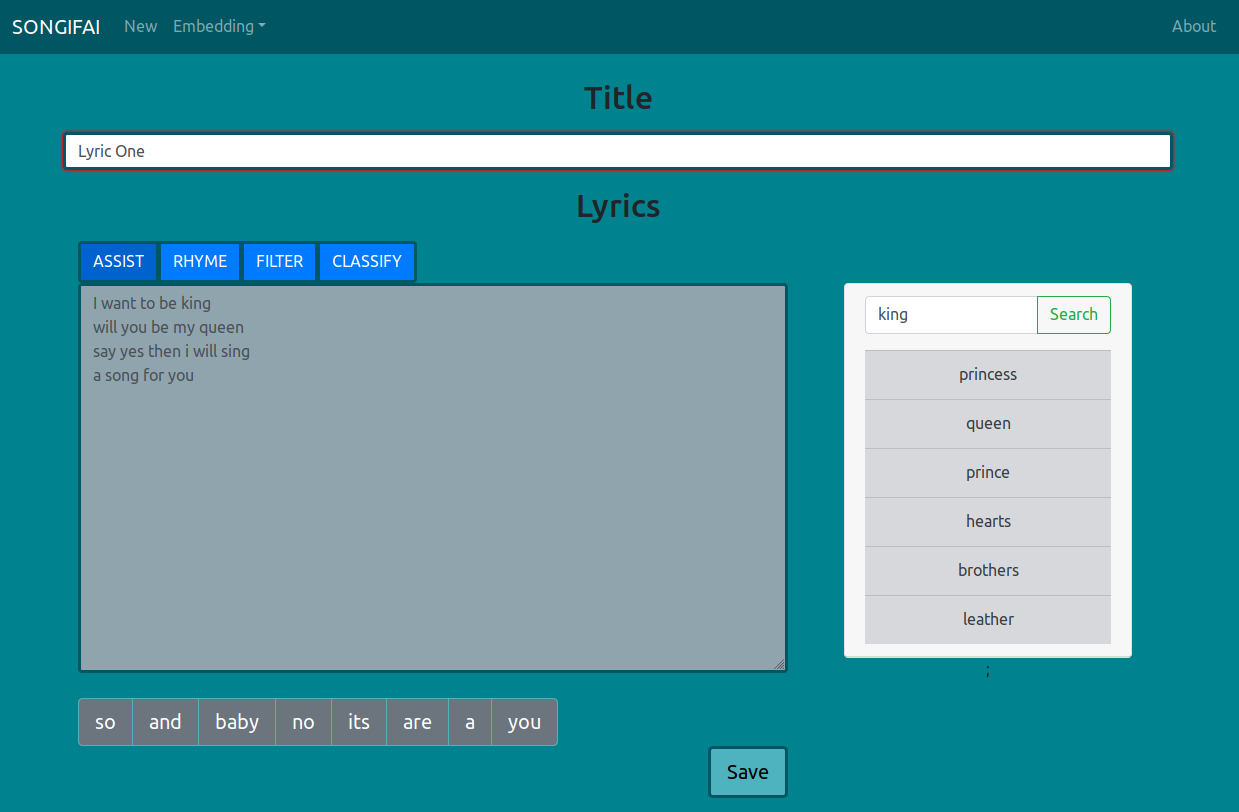
\includegraphics[width=13cm, height=9cm]{./figures/fig21}
	\caption[SONGIFAI Lyric Editor]{SONGIFAI Lyric Editor: Users can edit their lyrics and use the word prediction/suggestion features. Additional features such as explicit content filtering are also available.}
	\label{fig:songifaieditor}
\end{figure}

%%%%%%%%%%%%%%%%%%%%%%%%%%%%
% END DOCUMENT
\end{document}
%%%%%%%%%%%%%%%%%%%%%%%%%%%%